% UQ Gemini theme
% See: https://github.com/alfurka/gemini-uq
% Forked from
% https://rev.cs.uchicago.edu/k4rtik/gemini-uccs
% which is forked from
% https://github.com/anishathalye/gemini
%"L'argent, c'est une ressoyrce particulière, car on peut la transformer en n'importe quelle autre autre ressource". 
% Plot curve with an average reward probability => 3 curves
% Quand $S$ tend vers 0, $\beta = 1$, à vérifier en incluant $I(b)$. 
\documentclass[final]{beamer}
% ====================
% Packages
% ====================
\usepackage[T1]{fontenc}
\usepackage{lmodern}
\usepackage[size=custom,width=70.73,height=100,scale=1.0]{beamerposter}
\usetheme{gemini}
\usecolortheme{MVA}
\usepackage{graphicx}
\usepackage{booktabs}
\usepackage{tikz}
\usepackage{pgfplots}
\pgfplotsset{compat=1.17}
\newcommand{\N}{\mathbb{N}}
\newcommand{\Z}{\mathbb{Z}}
\newcommand{\R}{\mathbb{R}}
\newcommand{\C}{\mathbb{C}}
\newcommand{\E}{\mathbb{E}}
\newcommand{\Proba}{\mathbb{P}}
\usepackage[backend=biber, style=authoryear-comp]{biblatex}
\usepackage{csquotes}
\addbibresource{Bibliographie.bib}
% ====================
% Lengths
% ====================
% If you have N columns, choose \sepwidth and \colwidth such that
% (N+1)*\sepwidth + N*\colwidth = \paperwidth
\newlength{\sepwidth}
\newlength{\colwidth}
\setlength{\sepwidth}{0.025\paperwidth}
\setlength{\colwidth}{0.3\paperwidth}
\newcommand{\separatorcolumn}{\begin{column}{\sepwidth}\end{column}}
% ====================
% Title
% ====================
\title{Waltz right turn with a Humanoid Robot using Inverse Kinematics}
\author{Constantin Vaillant-Tenzer \inst{1} \inst{3} \and Charles Monte \inst{2} \inst{3} } %Authors name
\institute[shortinst]{\inst{1} Ecole Normale Supérieure - PSL \samelineand \inst{2} Telecom Paris \samelineand \inst{3} Master MVA}
% ====================
% Footer (optional)
% ====================
\footercontent{
  % \href{https://www.normalesup.org/$\sim$tenzer/}{www.normalesup.org/~tenzer} \hfill %Can also be your personal website
  MVA Robotics course, Final poster session, December 5 2024 \\ 
  \href{mailto:constantin.tenzer@ens.psl.eu}{constantin.tenzer@ens.psl.eu} \hfill \href{mailto:constantin.tenzer@ens.psl.eu}{charles.monte@telecom-paris.fr}}
% (can be left out to remove footer)
% ====================
% Logo (optional)
% ====================
% use this to include logos on the left and/or right side of the header:
% \logoright{\includegraphics[height=7cm]{logo1.pdf}}
% \logoleft{\includegraphics[height=7cm]{logo2.pdf}}
% ====================
% Body
% ====================
\begin{document}
\addtobeamertemplate{headline}{}
{
    \begin{tikzpicture}[remember picture,overlay]
      \node [anchor=north west, inner sep=3cm] at ([xshift=-1.0cm,yshift=-3.0cm]current page.north west)
      {
\includegraphics[height=5.0cm]{logos/logoDEC-rec.png} 
\includegraphics[height=5.0cm]{logos/logoLNC2_transp.png}}; % also try shield-white.eps
      \node [anchor=north east, inner sep=3cm] at ([xshift=1.2cm,yshift=-2cm]current page.north east)
      { 
\includegraphics[height=6.0cm]{logos/logoUP_inv.png}   
\includegraphics[height=5.0cm]{logos/logo_Inserm_inv.png}}; %add here logos for your other affiliations %
\includegraphics[height=4.5cm]{logos/logo_ens_psl_blanc_500px.png} 
    \end{tikzpicture}
}
\begin{frame}[t]
\begin{columns}[t]
\separatorcolumn
\begin{column}{\colwidth}
  
  \begin{block}{Introduction}
Our aim is to code a robot able to dance a waltz right turn using \textbf{inverse kinematics}.  
  
    \heading{Previous works}  
Waltz dancing is not a common research topic among dancing robots. However, to help robots learn how to dance, there are some already known methods like \textbf{learning from observation}(\cite{traditional_jap_dance}) where the robot chooses from a series of leg tasks the good ones to imitate a dancing human; or \textbf{real-time gesture responsive frameworks}(\cite{spectacle_imitation}) where the robot generates unpredictable artistic responses to a dancer's movements. \\ Concerning waltz dancing, a \textbf{dance partner robot}(\cite{ballroom_dance}) has been developed to realize human-robot coordination by estimating the next intended movement of a human through physical interaction.
  \end{block}

  \begin{block}{The waltz right turn movement in theory}
The movement made during a right turn of the waltz dance can be well described using the movement of the center of gravity of the person dancing. \\ During the dance, the person's movement is split in two summed parts: while moving along the perimeter of an ellipse - most commonly referenced as \textbf{the ball circle} - the dancer turns on himself along the perimeter of a circle with a diameter close to 1 meter. Both those translations can be estimated to be of constant angular velocities. \\ The dancer does a full turn around the circle every 360 beats of the music (of known BPM) so the angular velocity around the circle is $\omega_C = \frac{-2\pi \text{BPM}}{6*60}$ while we estimate the dancer to go around the ball room every minute, meaning the angular velocity around the ellipse is $\omega_E = \frac{-2\pi}{60}$. \\ The movement of the center of gravity we aim at reproducing looks like this from above. It has been simulated for 2 minutes with a 187 BPM music.
    \begin{figure}
      \centering
      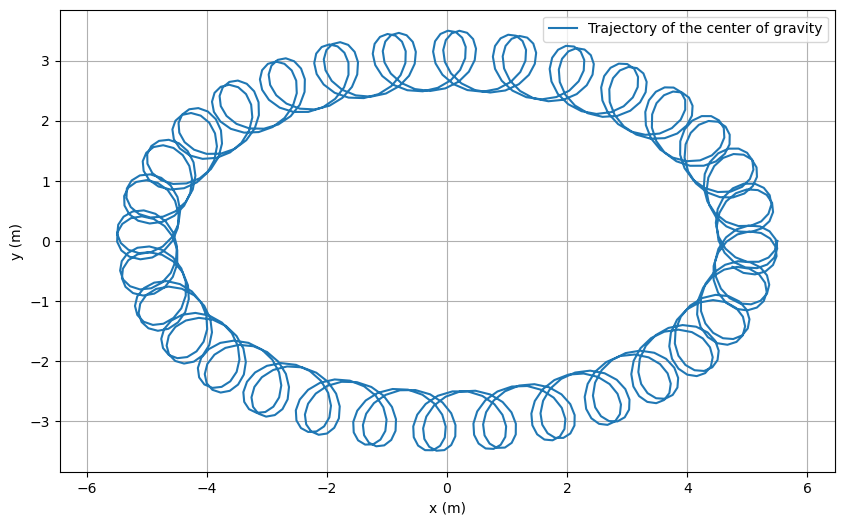
\includegraphics[width = 0.99 \columnwidth]{img/waltz_cog_movement.png} 
      \caption{Simulated movement of a Waltz dancer's center of gravity for 2 minutes}
    \end{figure}
  \end{block}
 \begin{alertblock}{Our approach of the problem}
To simulate the trajectory done by a dancer with a robot, we have trained a humanoid robot to follow the sequence of movements done by the dancer during a waltz right turn. \\ To do so, we first had to make the assumption that gravity and other forces applied to the dancer does not affect their movement. We also noticed that robots do not have to produce an effort to keep their chest upright, which means a robot will lead the movement with its feet, while humans do the opposite. Thus, the rotations will exclusively be produced thanks to the lower half of the robot body. \\
We then had to acquire the kinematics of the waltz right turn with the help of a video and then solve inverse kinematics with a humanoid robot model to fit the acquired movement. After having a robot able to dance the waltz right turn, we only had to fit the robot's movement to the music BPM, by making sure a right turn had the right duration.
 \end{alertblock}
 
\end{column}
\separatorcolumn
\begin{column}{\colwidth}
 \begin{block}{Our approach's pipeline}
  We did not have sufficient time to implement everything ourselves from kinematics acquisition to inverse kinematics solving so we decided to center ourselves around acquiring a good base for the movement kinematics. Thus, we mainly relied on already implemented blocks to fit inside our pipeline while trying to get the best approximation of a waltz right turn possible. \\ The global pipeline we followed for our implementation is the following.
  
    \begin{figure}
      \centering
      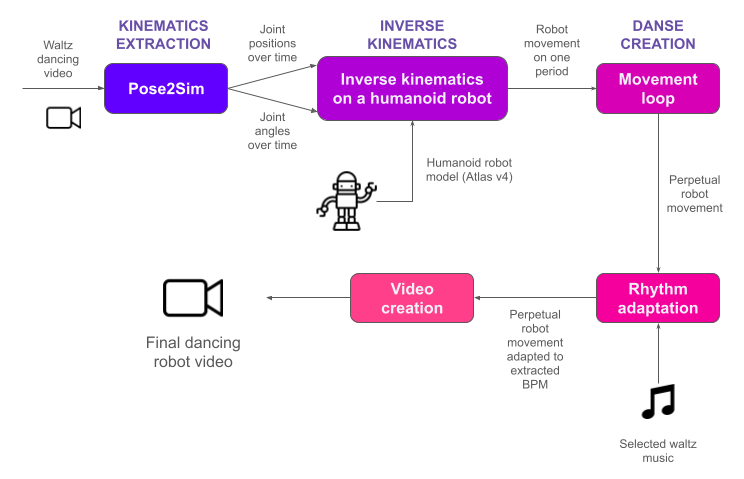
\includegraphics[width = 0.99 \columnwidth]{img/solution_pipeline.png}
      \caption{Our approach's full pipeline}
    \end{figure}
    
  \end{block}
  
\begin{block}{Already implemented blocks used}
 \heading{Kinematics acquisition}
After unsuccessful attempts to extract from proposed (\cite{Li_2019}), or discovered (\cite{li2023niki}) solutions both the joint positions and angles, we decided to use a pipeline that can extract both, \textbf{Pose2Sim} (\cite{Pose2Sim}). 
 \begin{figure}
      \centering
      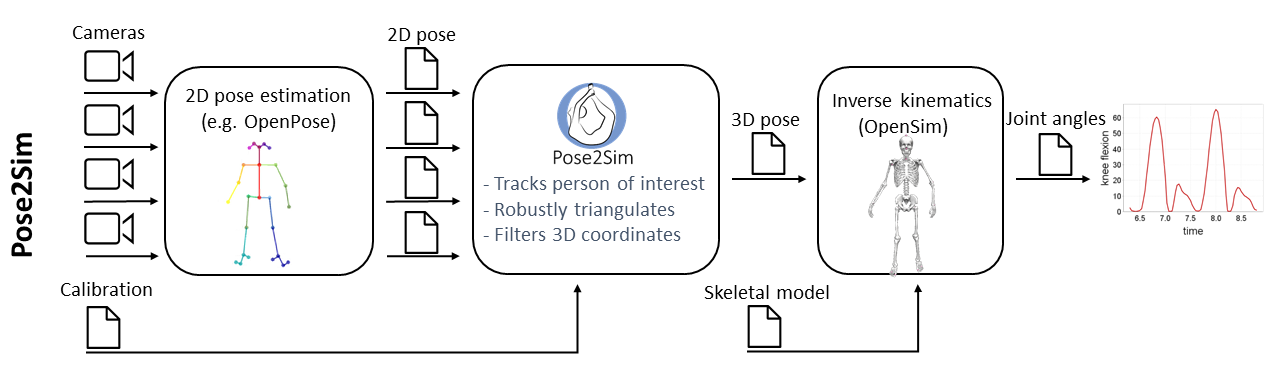
\includegraphics[width = 0.99 \columnwidth]{img/pose2sim_pipeline.png}
      \caption{The Pose2Sim pipeline}
    \end{figure}
\end{block}
This solution extracts 2D keypoints coordinates (using RTM Pose by \cite{RTMPose}) to produce an OpenSim result (full-body 3D joint angles), which we use in our pipeline by extracting the information that is interesting from us, ie. the RTMPose output and the full-body 3D joint angles. 

\heading{Inverse Kinematics solving}
To solve the inverse kinematics, we applied Pink (\cite{pink2024}) which solves differential inverse kinematics by weighted tasks. \\ 
The method uses \textbf{residual functions} of the robot configuration $q$ that should be driven to zero to make the robot do a certain task. In our case, we for instance try to put the robot's feet at a certain position $p_{\text{feet}}^*$ so an example of a residual would be $e(q) = p_{\text{feet}}^* - p_{\text{feet}}(q)$. \\
To solve the equation system produced, the method computes a velocity $v$ that satisfies the equation $J_e(q)v = \dot{e}(q) = -\alpha e(q)$ - $J_e(q)$ being the Jacobian of task $e$ - for each residual. It is of course not possible so the method finds the optimal solution to the following minimization problem, which finds the movement which tries to solve all of the tasks at the same time.
$$
\begin{aligned}
\min_v \ \ &\sum_{\text{tasks} \ e} ||J_e(q)v + \alpha e(q)||^2 \\
\text{subject to} \ \ \ &v_{min}(q) \leq v \leq v_{max}(q)
\end{aligned}
$$

\heading{Choice of a humanoid robot model}
We explored the Robot descriptions in Python repo (\cite{robot_descriptions_py}) to find a humanoid robot with similar joints to our Pose2Sim output, we finally decided to use AtlasV4 as our humanoid model.
  \end{column}
\separatorcolumn
\begin{column}{\colwidth}
  
  \begin{alertblock}{Our results}
  \end{alertblock}

  \begin{block}{Next steps}
While the results already are satisfying, we identified two further steps that could be added to the pipeline to achieve even better results :
\begin{enumerate}
    \item Adding a controlling module to maintain a constant angular velocity on the small circle. This cannot be done by humans and will make the movement look even better.
    \item Take care of the robot's balance throughout the movement.
\end{enumerate}
  \end{block}
  \begin{block}{References}
  %  \nocite{*}
%    \footnotesize{\bibliographystyle{plain}\bibliography{poster.bib}}
 \footnotesize{\printbibliography}
 %\printbibliography
 
  \end{block}
\end{column}
\separatorcolumn
\end{columns}
\end{frame}
\end{document}
